\documentclass[12pt]{article}
\usepackage[margin=1 in]{geometry}
\usepackage{graphicx}
\usepackage{float}
\usepackage{booktabs}
\usepackage{siunitx}
\usepackage{amsmath}


\title{Lab 9: Introduction to RC Circuits in the Time and Frequency-Domains}
\author{Sean Balbale}
\date{November 8th, 2024}
\setlength{\parindent}{0in}

\begin{document}

\begin{titlepage}
	\begin{center}
		\vspace*{1in}

		\Huge
		\textbf{Lab 9}

		\LARGE
		Introduction to RC Circuits in the Time and Frequency-Domains

		\vspace{3 in}

		\textbf{Student Name:} Sean Balbale
		\\ \textbf{Instructor:} Dr. Iman Salama
		\\ \textbf{Lab Partner Name:} Krish Gupta
		\\ \textbf{Date:} November 8, 2024

		\vfill


	\end{center}
\end{titlepage}

\newpage

\section{Introduction} 
This lab explored the behavior of RC (resistor-capacitor) circuits in 
time and frequency domains to understand their response to different 
input signals, essential in applications like signal processing and 
filtering. In Section \ref{subsec:part 1}, the transient response of 
an RC circuit was 
investigated using a square wave input to observe the exponential 
charging and discharging of the capacitor, governed by the time 
constant \(\tau = RC\). Adjustments in input frequency enabled full 
charge and discharge cycles, revealing insights into the circuit's 
time-domain behavior. Section \ref{subsec:part 2} analyzed the frequency 
response with a 
sine wave input across various frequencies, demonstrating 
frequency-dependent changes in output voltage magnitude and phase 
shift. These findings provided a foundational understanding of 
RC circuits’ responses across different conditions.


\section{Results}
% \begin{figure}[H]
% 	\centering
% 	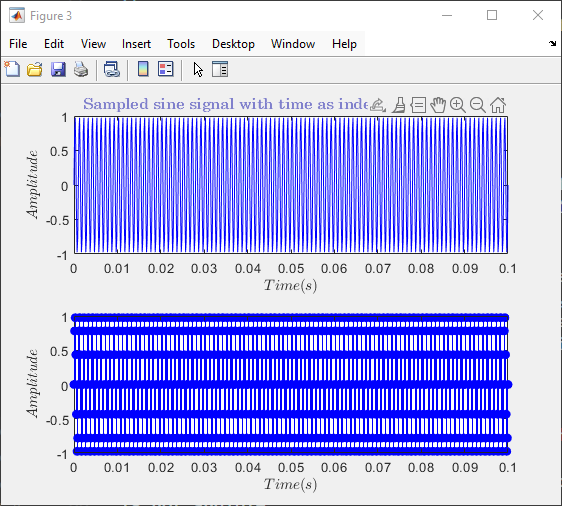
\includegraphics[width=0.3\textwidth]{fig 1f 7000.png}\hfill
% 	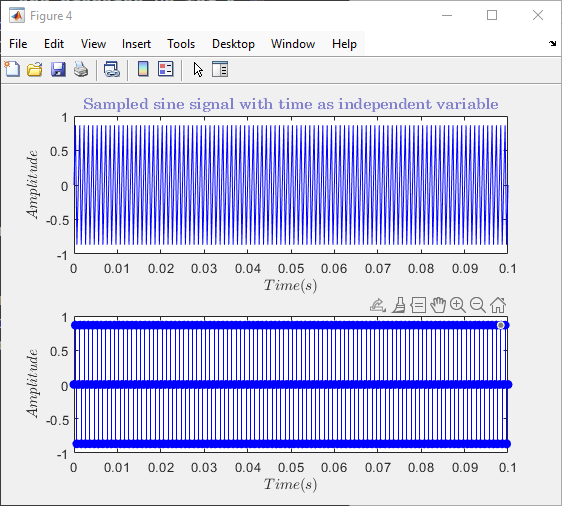
\includegraphics[width=0.3\textwidth]{fig 1f 3000.png}\hfill
% 	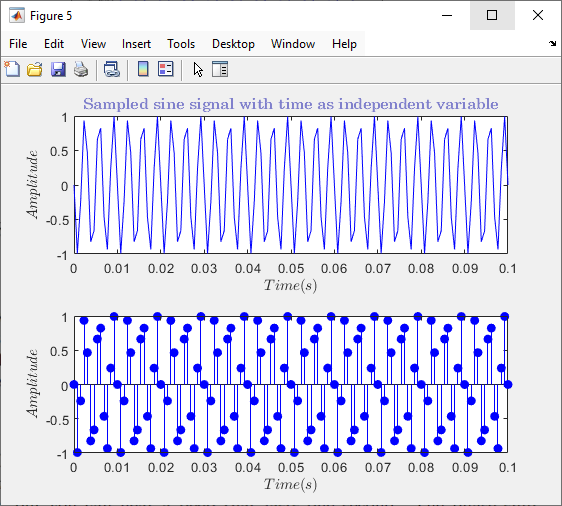
\includegraphics[width=0.3\textwidth]{fig 1f 1300.png}
% 	\caption{Sinusoidal with $f_s$ = 7 kHz, 3 kHz, and 1.3 kHz}
% 	\label{fig:fig3}
% % \end{figure}
\subsection{Transient Signals with an RC Circuit with Square Waves} \label{subsec:part 1}


\subsection{A Simple RC Circuit with Sine Waves} \label{subsec:part 2}

\section{Discussion and Conclusion}
\section{References}
 [1] Dr. Iman Salama. “Lab 9 – Introduction to RC Circuits in the Time and Frequency-Domains” Northeastern University. 8 November 2024.

\end{document}
